\begin{samplecase}
{\bf Medical isotope production with p + ${}^{100}$Mo}\newline
In this sample case, the activity of all the produced isotopes from the 
reaction p + ${}^{100}$Mo are given, for a 150 $\mu$A proton accelerator, as a function of time.
The following input file is used

\VerbatimInput{\samples p-Mo100-medical/org/talys.inp}

Note the use of the {\bf energy} keyword: Cross sections 
are calculated for incident energies between 8 and 30 MeV with 0.5 MeV 
energy steps. The keyword {\bf production y} means that activities of all 
radioactive products as a function of bombarding and/or decay time will be 
produced in tables. The incident energy of the particle beam is 24 MeV, and
the required thickness of the target (which is given in the output) is such that at the 
back of the target the energy is 10 MeV. Other keywords relevant for isotope 
production, such as 
{\bf Tcool}, see page \pageref{key:Tcool},
{\bf Tirrad}, see page \pageref{key:Tirrad},
{\bf rho}, see page \pageref{key:rho},
{\bf area}, see page \pageref{key:area},
{\bf radiounit}, see page \pageref{key:radiounit},
{\bf yieldunit}, see page \pageref{key:yieldunit},
have their default values in this sample case.

We like to point out an efficient option for medical isotope calculations. 
Suppose one is interested in varying several accelerator options, 
such as e.g. {\bf Ebeam}. Once the first calculation, like the sample case 
above, has been done, one may rerun that case and add the extra line 
{\bf reaction n} to the input file. 
Then, TALYS will {\it not} redo the nuclear reaction calculations, but use the 
various {\it rpZZZAAA.tot, etc.} cross section output files which are already available in the work 
directory. Obviously, {\bf Ebeam} and {\bf Eback} must always fall inside the energy 
grid for which the cross sections are calculated, in this case between 8 and 30 MeV.

Of most interest are probably the files with the produced activity (in Bq or Ci) per
isotope. These yields are in files
{\em YZZZAAA.tot} where ZZZ is the charge number and AAA is the mass number in
(i3.3) format. For produced isomers, and ground states, 
there are additional files {\em pZZZAAA.LMM}, where MM is the number
of the isomer (ground state=0) in (i2.2) format.
For the above sample case, {\it Y043099.L02}, i.e. the production of ${}^{99m}$Tc
looks as follows:
{\small \begin{verbatim}

# header:
#   title: Mo100(p,x)Tc99m Isotope production
#   source: TALYS-2.0
#   user: Arjan Koning
#   date: 2023-12-14
#   format: YANDF-0.1
# target:
#   Z: 42
#   A: 100
#   nuclide: Mo100
# reaction:
#   type: (p,x)
# residual:
#   Z: 43
#   A: 99
#   nuclide: Tc99m
# parameters:
#   Beam current [mA]:  1.500000E-01
#   E-Beam [MeV]:  2.400000E+01
#   E-Back [MeV]:  1.000000E+01
#   Initial production rate [s^-1]:  1.961665E-10
#   Decay rate [s^-1]:  3.203675E-05
#   Initial production yield [GBq/mAh]:  2.119981E-01
#   Total activity at EOI [GBq]:  9.572902E+02
#   Irradiation time:       0 years   1 days  0 hours  0 minutes  0 seconds
#   Cooling time:       0 years   1 days  0 hours  0 minutes  0 seconds
#   Half-life:       0 years   0 days  6 hours  0 minutes 36 seconds
#   Maximum production at:       0 years   3 days 16 hours 36 minutes 54 seconds
# datablock:
#   quantity: Isotope production
#   columns: 5
#   entries: 100
##     Time         Activity       Isotopes         Yield     Isotopic fract.
##      [h]           [GBq]           []            [GBq]           []
   5.000000E-01   5.723950E+01   1.786682E+15   2.119981E-01   9.946191E-02
   1.000000E+00   1.112715E+02   3.473244E+15   2.001184E-01   9.695597E-02
   1.500000E+00   1.622756E+02   5.065295E+15   1.889043E-01   9.452177E-02
   2.000000E+00   2.104216E+02   6.568132E+15   1.783186E-01   9.216321E-02
   2.500000E+00   2.558697E+02   7.986755E+15   1.683262E-01   8.987931E-02
...................................
\end{verbatim} } \renewcommand{\baselinestretch}{1.07}\small\normalsize
\noindent
where the final column denotes the fraction of the produced isotope relative to all 
isotopes of that element. Fig. \ref{tc99m} shows the $^{99m}$Tc production as a function of time.
Note that the curve is not  a straight line due to the decay of $^{99m}$Tc to 
the ground state.
\end{samplecase}
\begin{figure}
\centering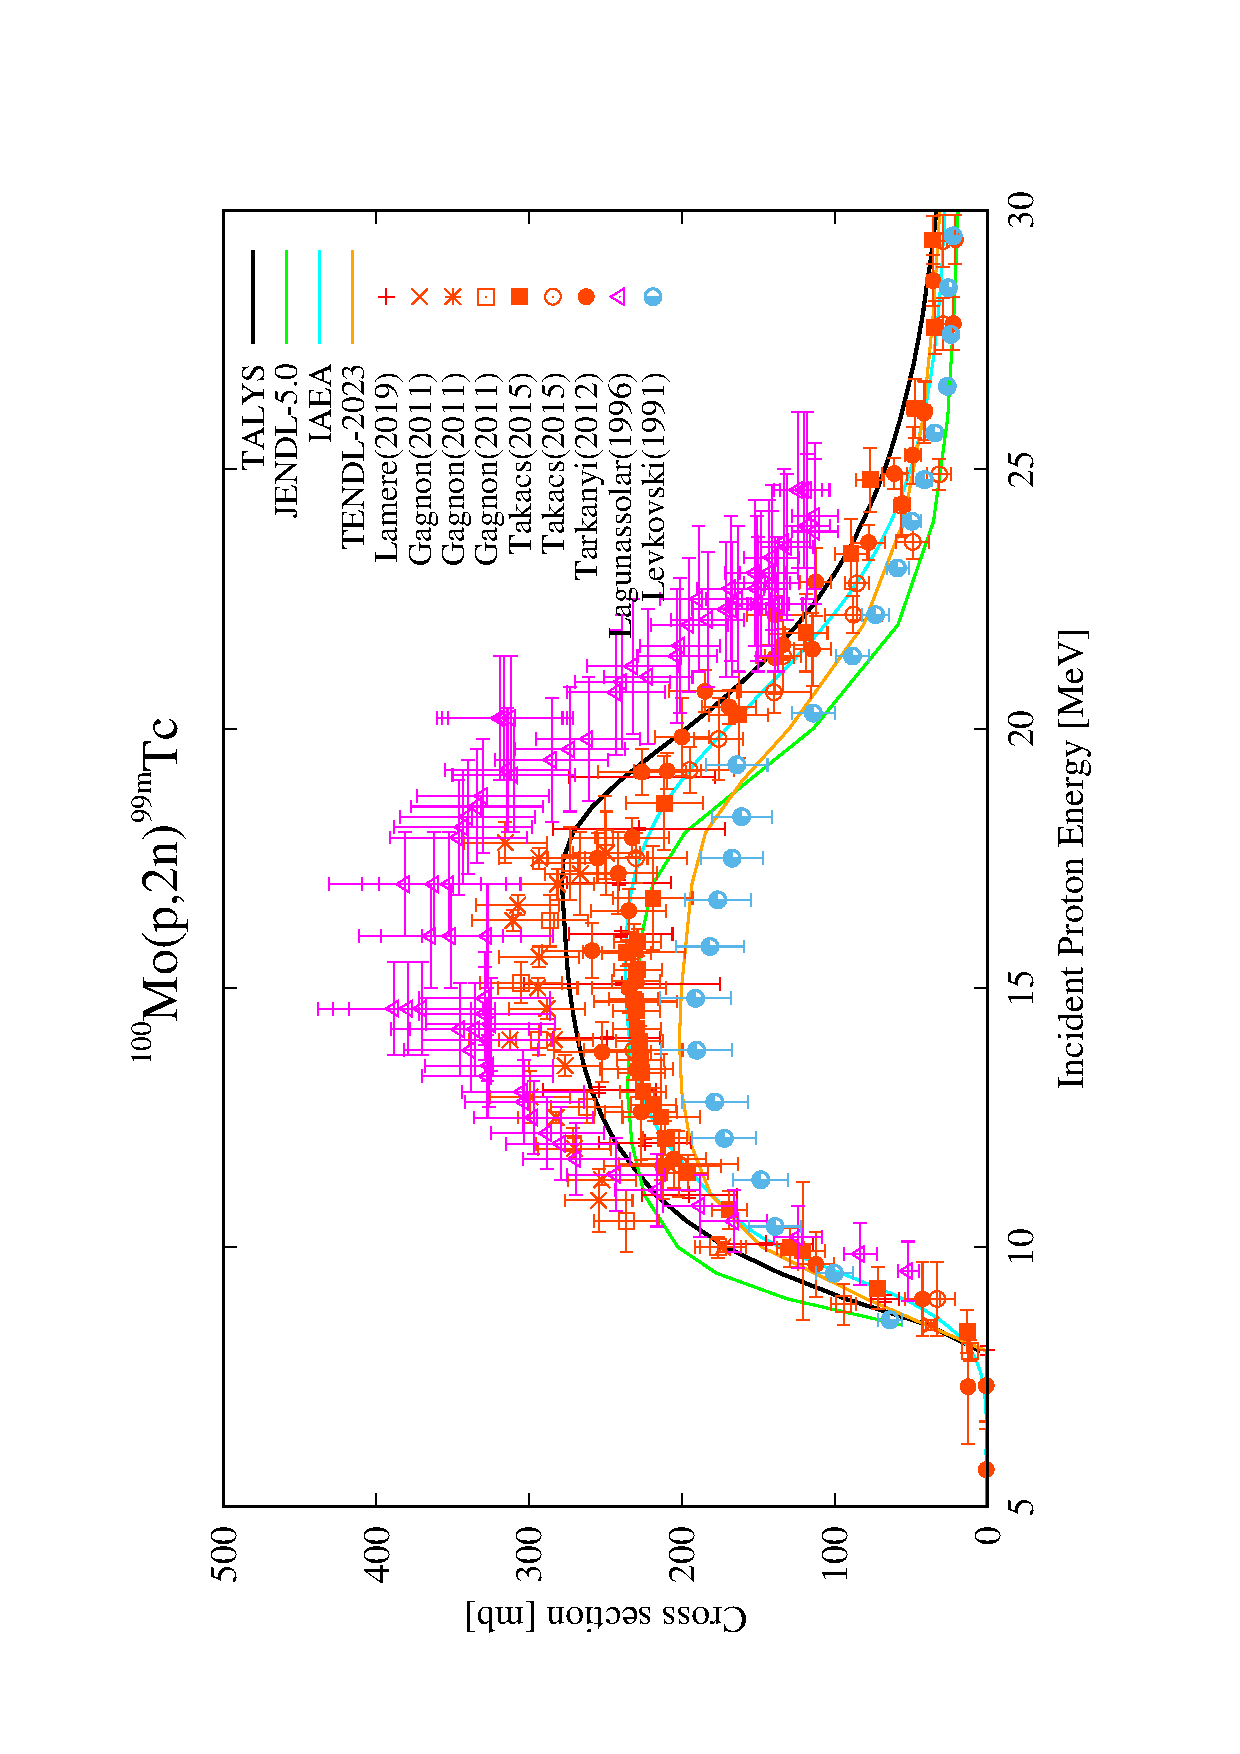
\includegraphics[scale=0.5,angle=270]{p-Mo100-p2n}
\caption{Excitation function of $^{100}$Mo(p,2n)$^{99m}$Tc.}
\label{tc99mcross}
\end{figure}
\begin{figure}
\centering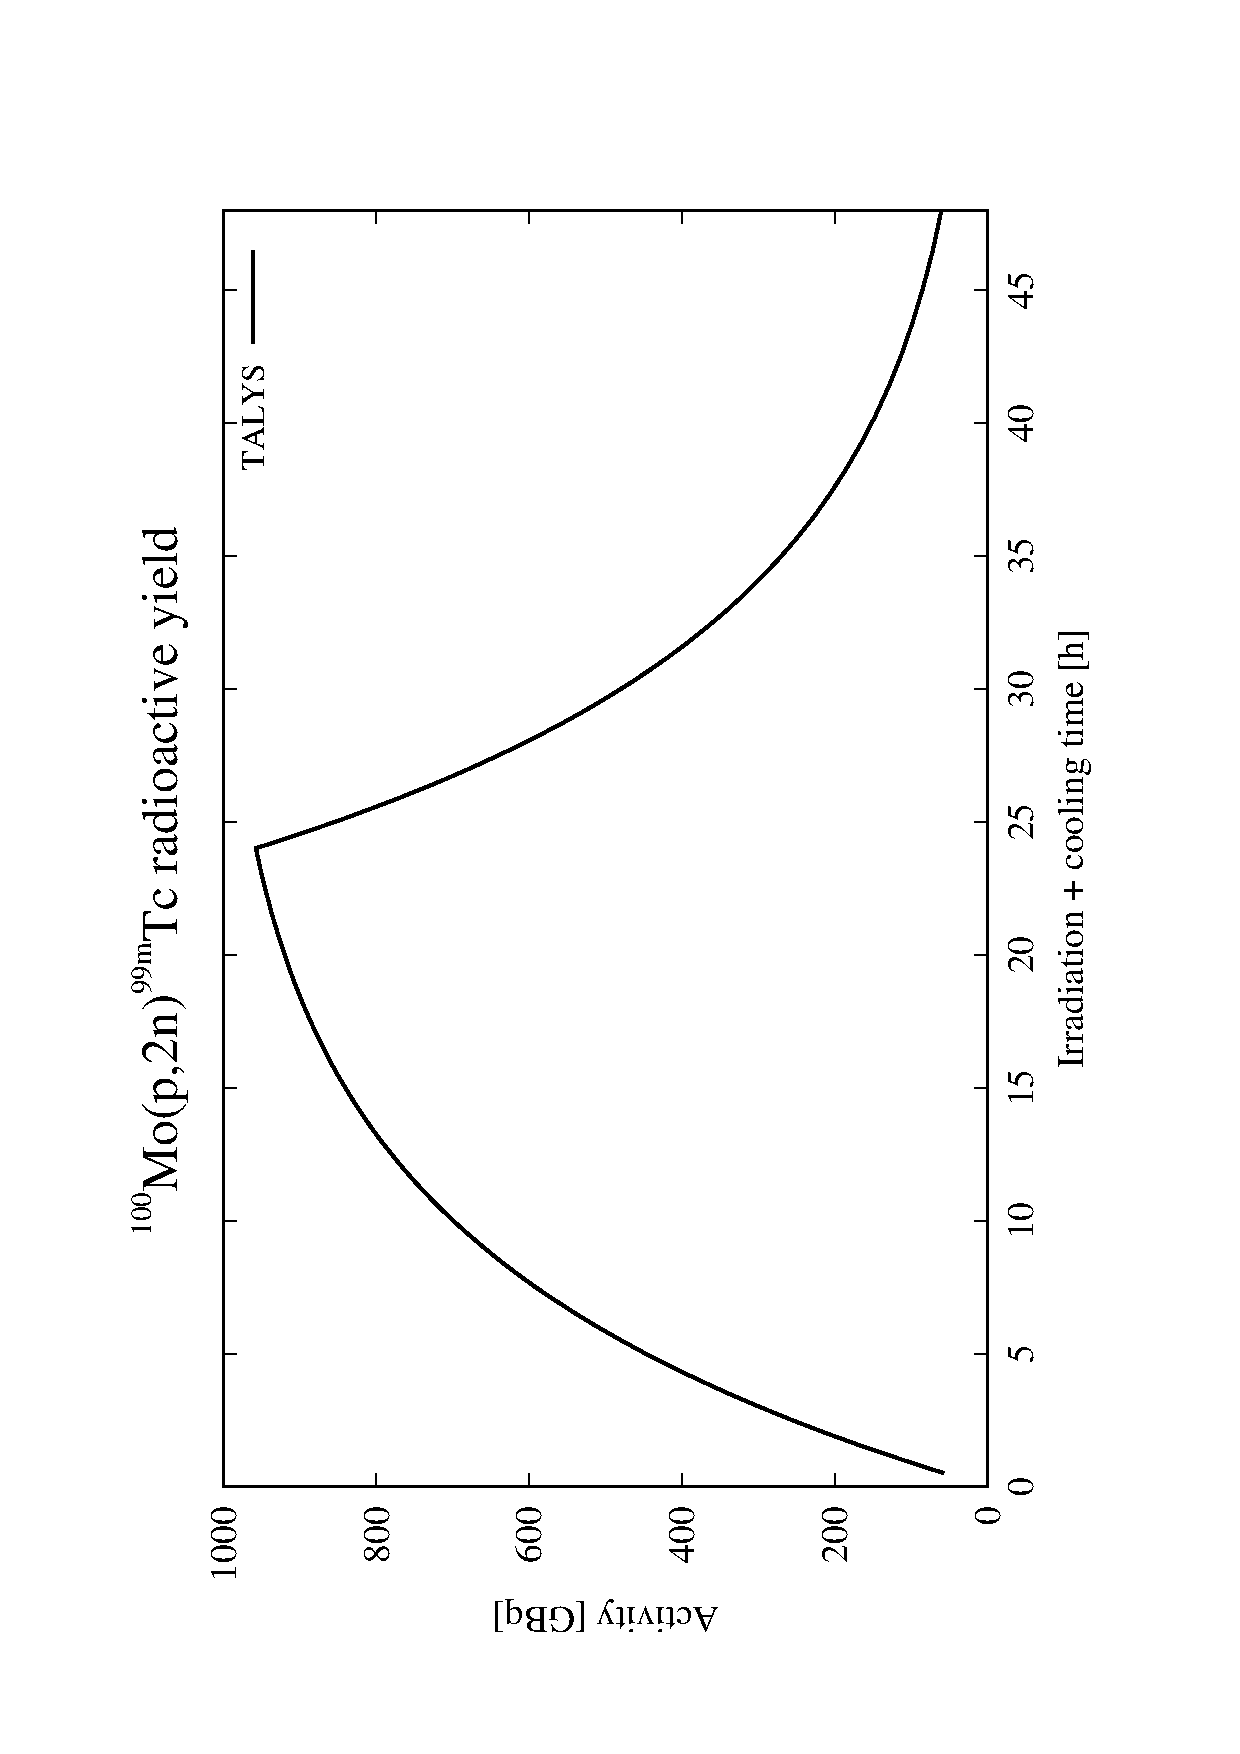
\includegraphics[scale=0.5,angle=270]{p-Mo100-yield}
\caption{Total activity of $^{99m}$Tc produced by a 24 MeV proton accelerator of 
150 $\mu$A and a $^{100}$Mo target with an energy of 10 MeV at the back of the 
target.}
\label{tc99m}
\end{figure}
